\chapter{Future Work \& Planning}
\label{cha:planning}

\section{Intro}
\label{sec:planningIntro}

The initial stage of this project was
completed with another 4 curricular units,
focusing on finding usable datasets for 
a replication of \gls{eRange} estimation
through "basic" \gls{SOC} based estimation, 
and adaptive history based model approaches.
Additional research on of existing related works,
has also been executed for better understanding
of the problem regarding \gls{eRange} estimation
and its difficulties.

\section{Planning}
\label{sec:planningPlanning}

\begin{figure}[H]
    \begin{center}
        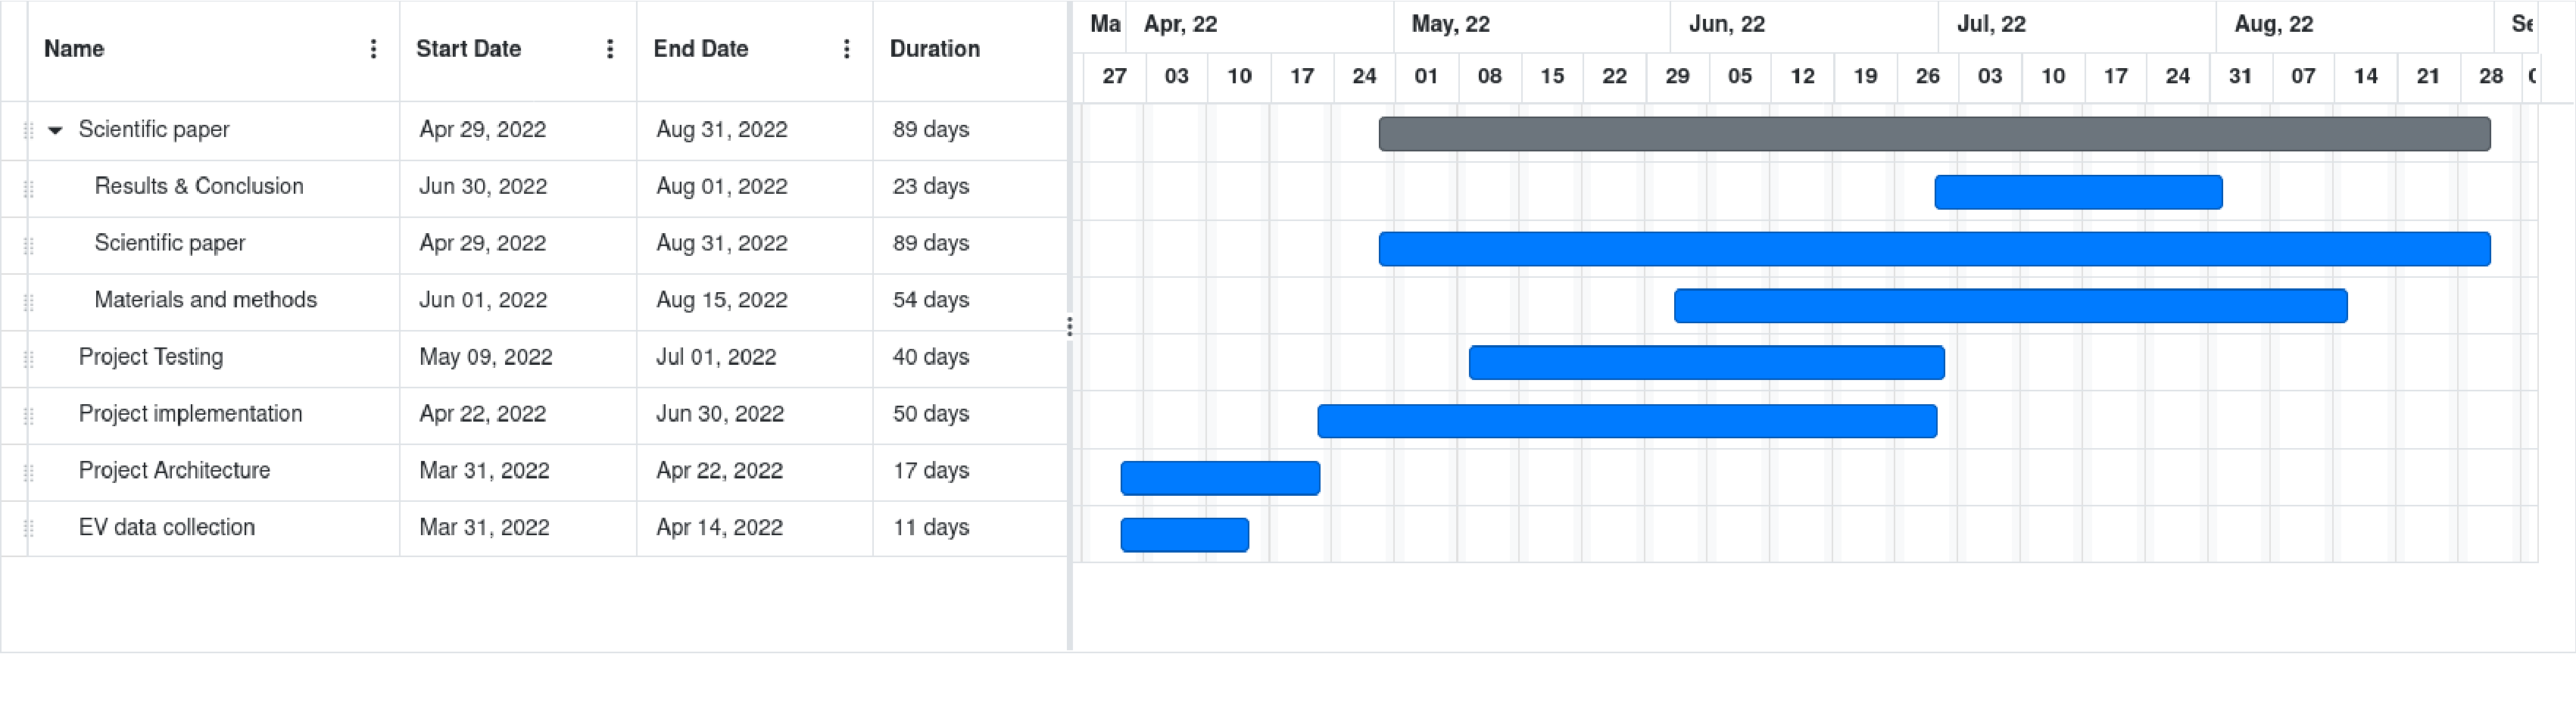
\includegraphics[scale=0.27]{../figures/planning}
        \caption{Project planning.}
    \end{center}
\end{figure}